
\mychapter{The Risch Theorem}

{\bf THIS CHAPTER IS VERY VAGUE AND INCOMPLETE.}

We now turn to the task of proving the Risch theorem.

There are three key steps in this proof.

\begin{enumerate}

\item Establish the existence of the Jacobian variety.

It's not that hard to see that divisor classes on an algebraic curve
can be composed and inverted, forming the {\it divisor class group}.
It's not nearly so obvious that these divisor classes can be
identified with the points on an algebraic variety.  The resulting
{\it Jacobian variety} is thus both a group and an algebraic variety,
and the group operations can be represented by rational functions on
the algebraic variety, thus forming an {\it Abelian variety},
which is an algebraic variety equipped with a group structure.

\item Prove that the following diagram commutes:

\begin{center}
\Large
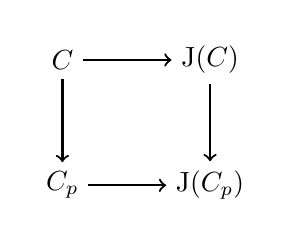
\begin{tikzpicture}
\matrix [column sep=10mm,row sep=10mm]
{
\node (C) {$C$}; & \node (JC) {J($C$)}; \\
\node (Cp) {$C_p$}; & \node (JCp) {J($C_p$)}; \\
};
\draw [thick, ->] (C) -- (JC);
\draw [thick, ->] (Cp) -- (JCp);
\draw [thick, ->] (C) -- (Cp);
\draw [thick, ->] (JC) -- (JCp);
\end{tikzpicture}
\end{center}

The objects on the left are algebraic curves; the objects on the right
are Abelian varieties.  The horizontal arrows correspond to constructing
a curve's associated Jacobian variety; the vertical arrows correspond
to reduction modulo a prime.

At the end of the previous chapter, we were working on the lower-left
half of this diagram.  We reduced a curve modulo a prime, then computed
the order of various divisors on the reduced curve, which essentially
computes orders of points on the reduced curve's Jacobian variety.
We now wish to show that those group orders are the same as if we
had constructed the Jacobian of the original curve and then reduced
the Jacobian modulo the prime.

\item Study the effects of reduction modulo a prime on an Abelian variety.

At this point, we no longer need any special properties of the
Jacobian variety; it suffices to study how reduction modulo a prime
affects the group structure on an Abelian variety.  In particular, we
will find that the factor of an element's order coprime to the
reduction prime is preserved.

\end{enumerate}

\section{The Riemann-Roch Theorem}

The Riemann-Roch Theorem is one of the most celebrated theorems in
mathematics.  Not only does it provide a crucial tool in understanding
the structure of algebraic extensions, but it does so by tying
together algebra, analysis, and geometry in one equation.

First, let's review that equation:

\theorem {\rm (Riemann-Roch)}

% For any divisor $\mathfrak{b}$,
% 
% $$l(\mathfrak{b}) = \deg \mathfrak{b} + 1 - g + l(\mathfrak{c}-\mathfrak{b}) $$
% 
% where $l(\mathfrak{b})$ is the dimension of the vector space
% $L(\mathfrak{b})$ of multiples of $-\mathfrak{b}$, $g$ is the genus of
% the extension, and $\mathfrak{c}$ is any divisor of the canonical class of
% differentials.

For any divisor $\mathfrak{b}$,

% $$l(\mathfrak{b}) = \deg \mathfrak{b} + 1 - g + l(\mathfrak{c}-\mathfrak{b}) $$
% $$l(-\mathfrak{b}) = \deg \mathfrak{b} + 1 - g + l(\mathfrak{b}-\mathfrak{c}) $$
% $$l(\mathfrak{b}) = \deg -\mathfrak{b} + 1 - g + l(-\mathfrak{b}-\mathfrak{c}) $$
% $$l(\mathfrak{b}) = - \deg \mathfrak{b} + 1 - g + l(-\mathfrak{b}-\mathfrak{c}) $$

$$l(\mathfrak{b}) = - \deg \mathfrak{b} + 1 - g + l(-\mathfrak{b}-\mathfrak{c}) $$

where $l(\mathfrak{b})$ is the dimension of the vector space
$L(\mathfrak{b})$ of multiples of $\mathfrak{b}$, $g$ is the genus of
the extension, and $\mathfrak{c}$ is any divisor of the canonical class of
differentials.

\endtheorem

Interrelated by this theorem is the purely algebraic concept of the
dimension of the vector space of multiples of a divisor, the geometric
concept of the genus, and the analytic concept of a differential.

However, this sophistication comes with a price.  Specifically, we
need a topology to define the genus, and we need a limit to define the
differential.

Andr\'e Weil showed how the Riemann-Roch theorem can be stripped of
the analysis and the geometry, and proved as purely a result in
algebra.  The genus, instead of a topological invariant, now appears
as merely a least upper bound on a divisor's degree of specialization,
and a differential becomes an object in a dual space that maps a
function into the field of constants.  The advantage of this
formulation is that does not require any topological structure, and is
therefore well suited to use with finite fields.  It is this
formulation I will now adopt.

First, at any place in the function field, there is a local valuation
ring with a maximal prime ideal.  We can normalize the valuation (it
is discrete) and pick a element of unit valuation to use as a
uniformizing variable.  By multiplying as necessary by some power of
this element, we can adjust any field element to be a unit of the
valuation ring and thus associate an order ${\rm ord}_{\mathfrak{p}}$
with that element.  The valuation ring's units are a finite extension
of the constant subfield; they are the constant subfield if it is
algebraically closed.  By subtracting out the remainder mod
$\mathfrak{p}$, we get an element of higher order, which we can again
subtract out, and so on, building a power series in the uniformizing
variable.  Each element of the function field thus has a power series
associated with it at each place $\mathfrak{p}$.

A collection of such power series, one at each place, with arbitrary
coefficients except that there are only a finite number of
coefficients with negative powers, is called a {\it vector}.  Each
individual power series is called a {\it component} of the vector.
Clearly, every function has a vector associated with it; but the
converse is not necessarily true.  The mapping from functions to
vectors is injective, though.  Any two different functions will have a
non-zero difference that must therefore have a finite value, of finite
order, at some place $\mathfrak{p}$, and their vectors will differ at
that point.

We also have a dual space of {\it covectors}.  The coefficients of a
covector component at a place are dual to the constant field at that
place; if the constant field is algebraically closed, then the
covector coefficients are in the constant field.  Like vectors,
covectors can only have a finite number of negative power
coefficients.

We define a dot product between a vector $v$ and a covector $\lambda$:

$$ v \cdot \lambda = \sum_{\mathfrak{p}} \sum_{i+j=-1} v_{\mathfrak{p},i}
  \lambda_{\mathfrak{p},j} $$

where $v_{\mathfrak{p},i}$ is the coefficient of the $i^{\rm th}$
power in $v$'s component at $\mathfrak{p}$, and likewise for
$\lambda_{\mathfrak{p},j}$.  Notice that the second summation requires
at least one of $i$ or $j$ to be negative, so there will only be a
finite number of places for the first sum at which the second sum
contributes anything at all.

Weil also requires the {\it Theorem of Independence}, which states
that, although an arbitrary (full) vector may not have a function
associated with it, a function can always be found which matches a set
of finite prefixes at a finite number of places.  This can be
demonstrated using Theorem \ref{finite orders construction},
repeatedly applied a finite number of times.  We also need to know
that a function without a pole is constant.

With this setup, we can now prove a series of theorems that lead up
the the Riemann-Roch Theorem.

\theorem

$$l(\mathfrak{p}) \leq \deg \mathfrak{p} +1$$

i.e, $l(\mathfrak{p})$, the dimension (over the constants) of
$L(\mathfrak{p})$, the multiples of $-\mathfrak{p}$, is no more than
the degree of the divisor $\mathfrak{p}$, plus one.

\proof

Since $\deg -\mathfrak{p} = - \deg \mathfrak{p}$, there are at least
$\deg \mathfrak{p}$ poles (counting multiplicities) in
$-\mathfrak{p}$, and at least $\deg \mathfrak{p}$
coefficients with negative powers in the vectors corresponding
to the elements in $L(\mathfrak{p})$

.  We can impose

\endtheorem

\theorem

If $\mathfrak{A}$ is divisible by $\mathfrak{B}$, i.e, if
$\mathfrak{A}\mathfrak{B}^{-1} \subseteq {\cal I}$, then

$$n(\mathfrak{A}) - l(\mathfrak{A}) \leq n(\mathfrak{B}) - l(\mathfrak{B}) $$

$$n(\mathfrak{p}) \equiv {\rm deg} \mathfrak{p}$$

\proof

Consider $\mathfrak{C} = \mathfrak{A}\mathfrak{B}^{-1}$.
Now $n(\mathfrak{C}) = n(\mathfrak{A}) - n(\mathfrak{B})$ and since
$\deg -\mathfrak{C} = - \deg \mathfrak{C}$, and
$\mathfrak{C}$ is integral (by supposition),
there are exactly
$n(\mathfrak{C})$ poles (counting multiplicities) in $-\mathfrak{C}$.
, and at least $\deg \mathfrak{p}$
coefficients with negative powers in the vectors corresponding
to the elements in $L(\mathfrak{p})$

.  We can impose

\endtheorem

It immediately follows (from $\mathfrak{b}={\bf 0}$) that
$l(\mathfrak{c})=g$, which can be taken as the definition of the
genus.



\section{Jacobian Varieties}

An algebraic extension is a simple example of what algebraic geometers
term a {\it variety}, which is the zero locus of a set of polynomials
defined over some field.  Thus, for example, the unit circle is a
variety (defined over the real numbers), because it is the zero locus
of $x^2+y^2=1$.  But the points $(1,0)$ and $(-1,0)$ are also a
variety, because they are the zero locus of the {\it set} of
polynomials $\{x^2=1; y=0\}$.

An {\it abelian variety} is a variety accompanied by a commutative
group structure on its elements, which typically includes picking an
arbitrary zero point as the identity element.  The circle is an
abelian variety, if we identify its points with their angles from the
x-axis and make $(1,0)$ our identity element.  Now any two points can
be ``added'' or ``subtracted'' (by adding or subtracting their
respective angles) to obtain a third point, and each point has an
inverse associated with it (its mirror image across the x-axis).  It
should be obvious that the choice of a zero point was totally
arbitrary.  Likewise, the points ${(1,0), (-1,0)}$ also form an
abelian variety; their group structure is isomorphic to ${\bf Z}_2$ and
the choice of one of them as the identity is, again, arbitrary.

Is every variety abelian?  No, but any complete, non-singular variety
can be homomorphicly mapped into an associated abelian variety
(typically of higher dimension), called its {\it Jacobian variety}.
This fact, combined with the extensive body of literature on abelian
varieties ([Mumford], [Birkenhake and Lange], [Lang], to mention a
few), makes the Jacobian variety an important object of study (though
David Mumford, in the preface to [Mumford], described it as a
``crutch'').

We will be needing only a tiny bit of this theory here, so my goal in
this section is only to demonstrate how the Riemann-Roch Theorem
allows us to set up an abelian group structures on an algebraic
extension.

The oldest construction of the Jacobian variety uses integrals
and only works over the complex field $\CC$, and requires us
to work on a non-singular model of the curve.

We can pick an arbitrary origin and $2g$ closed paths from that
origin that form a basis for the surface's holonomy group.
We can also pick $g$ independent holomorphic differentials
and evaluate them over the $2g$ closed paths to get a lattice
$\Lambda^g$ in $\CC^g$.  Given any point on the surface,
we can now evaluate the differentials along a path from
the origin to that point and thus map into the torus
$\CC^g/\Lambda^g$.

Not all complex torii are algebraic varieties, but this one is (PROOF
NEEDED).

Now, Abel's Theorem and the Jacobi inversion theorem ([Griffiths and
Harris], p. 235) shows that ${\rm Pic}^0$, the group of divisors of
degree zero modulo linear equivalence is isomorphic to
$\CC^g/\Lambda^g$.

Alternately, ([Lang], II, \S1, Theorem 3), we can factor a mapping
of a product into an abelian variety into mappings on each factor.

Lang also characterizes Abel's theorem as follows:

\begin{quote}

Let $\omega_1, ..., \omega_g$ be a basis for the differential forms
on the first kind of V.  If $\mathfrak{a} = \sum n_i P_i$ is a
[divisor] of degree 0 on V, and P is a fixed point of V, then
the map into ${\bf C}/\Lambda^g$ given by:

$$\mathfrak{a} \to \sum n_i (\int_P^{P_i}\omega_1, ..., \int_P^{P_i}\omega_g)$$

is well defined modulo the periods... the kernel consists of those
divisors that are linearly equivalent to 0 (i.e, principal); this is
Abel's theorem.

\end{quote}

Pulling this all together, we need to show that the group operation
is defined by rational functions.

For our purposes, it isn't enough to construct the Jacobian over the
complex field $\CC$; we also need Jacobians for curves in prime
characteristic.  So the traditional construction using integrals
isn't available, we need something different.

Andre Weil, in Courbes Algébriques et Variétés Abéliennes (1948),
constructs the Jacobian variety over arbitrary fields using the g-fold
symmetric product of the curve.  See Michel Raynaud, ``André Weil and
the Foundations of Algebraic Geometry'' for an broad overview of this
French text.

J.S. Milne's ``Jacobian Varieties'' (jmilne.org/math) also uses the
symmetric power of the variety.

Greg Anderson, ``Abeliants and their application to an elementary
construction of Jacobians'' uses equivalence classes of matrices
constructed using a Riemann-Roch space.  Equivalence of matrices
defined over a vector space, as Joshua Grochow taught me\footnote{\tt
https://mathoverflow.net/questions/303627}, is the same as
simultaneous equivalence of matrices, a notoriously hard problem.
Sergeichuk, ``Canonical matrices for linear matrix problems''
shows how to convert such a matrix into an canonical form,
but there's no obvious way to introduce the rank 1 condition
required by Anderson's construction, nor is the canonical form
easily parametized.




\section{Simple Algebraic Extensions over Finite Fields}

Let's start with a simple but crucial observation:

\theorem

In an algebraic extension over a finite field, the evaluation field is
also finite.

\proof

Consider a finite field of constants ${\cal F}$, over which we'll
extend first into a rational function field ${\cal F}(x)$ and then add
an algebraic extension ${\cal F}(x,y)$, where $y$ satisfies some
minimial polynomial $f(x,y)=0$.  Start with the constant field, which
gives us a finite number of values for $x$.  Plugging each of these
values into the minimal polynomial gives a finite set of polynomials
$f(y_i)=0$.  By Theorem ?, we can extend ${\cal F}$ into a finite
extension field ${\cal F}[\gamma]$ where all the roots of the
polynomial exist.  Since there a only a finite number of polynomials,
we need at worst a finite set of extensions ${\cal
F}[\gamma_1,...,\gamma_k]$ to construct a field in which all the roots
of all the polynomials exist.  Using the Theorem of the Primitive
Element, we can collapse all of these into a single finite extension
field ${\cal F}[\phi]$.  Since all values of $x$ exist in ${\cal F}$,
and all values of $y$ exist in ${\cal F}[\phi]$, an evaluation
homomorphism carries any rational function in $x$ and $y$ into
${\cal F}[\phi]$.

\endtheorem

This theorem leads directly to the single more important difference
(to us) between divisors in an infinite field versus those in a finite
field.  {\it In a finite field, some multiple of every divisor is
principal.}  The reason is that the multiplicative group of the
evaluation field has finite order.  The simplest way to demonstrate
this is to construct theorems analogous to Theorems ? and ?:

\theorem

In an algebraic extension of a finite field with characteristic
greater than 2, a function can always be constructed with an $m^{\rm
th}$-order zero at a specified place $(\alpha, \beta)$ and zero order
at all other finite places, where $m$ is the multiplicative order of
the evaluation field.

\proof

The desired function is

$$(x-\alpha)^m + (y-\beta)^m$$.

Clearly, this function is zero at $(\alpha, \beta)$ and of $m^{\rm
th}$ order there (PROOF THIS).  At all other places one of the two
terms will be non-zero, and both exist in the evaluation field.  By
Theorem ?, any non-zero number raised to the multiplicative order of
its field is one.  Thus the value of this function will be either
$1+0$, $0+1$, or $1+1=2$, all finite and non-zero, and thus of zero
order.

\endtheorem

\theorem

In an algebraic extension of a finite field with characteristic
greater than 2, a function can always be constructed with an $m^{\rm
th}$-order pole at a specified place $(\alpha, \beta)$ and zero order
at all other finite places, where $m$ is the multiplicative order of
the evaluation field.

\proof

The desired function is

$${f(\alpha,y)^m\over(x-\alpha)^m(y-\beta)^m} + 1$$

where the division by $(y-\beta)^m$ is exact.
Clearly, this function has a pole at $(\alpha, \beta)$ and of $m^{\rm
th}$ order there (PROOF THIS).  CONSIDER OTHER PLACES OVER $\alpha$.
At all other places the denominator
term will be non-zero, and thus one, and the numerator will be
either zero or one (by Theorem ?)
Thus the value of this function at these places will be either
$0+1$ or $1+1=2$, both finite and non-zero, and thus of zero
order.

\endtheorem


\example

Show that some multiple of ${\mathrm Z}(1,1)$ is principal in
${\bf Z}_5(x,y); y^2=x$.

Let's first construct a multiplication table for ${\bf Z}_5$:

\begin{center}
\begin{tabular}{c|c c c c c}
  & 0 & 1 & 2 & 3 & 4 \cr
\hline
0 & 0 & 0 & 0 & 0 & 0 \cr
1 & 0 & 1 & 2 & 3 & 4 \cr
2 & 0 & 2 & 4 & 1 & 3 \cr
3 & 0 & 3 & 1 & 4 & 2 \cr
4 & 0 & 4 & 3 & 2 & 1 \cr
\end{tabular}
\end{center}

Now, let's list out the places on the Riemann surface for
${\bf Z}_5(x,y); y^2=x$.

\begin{center}
\begin{tabular}{c l}
$x$ & $(x,y)$ \cr
\hline
0 & (0,0) \cr
1 & (1,1) \quad (1,4) \cr
2 & $(2,\gamma) \quad (2,-\gamma); \quad \gamma^2 - 2 =0$ \cr
3 & $(3,\theta) \quad (3,-\theta); \quad \theta^2 - 3 =0$ \cr
4 & (4,2) \quad (4,3) \cr
\end{tabular}
\end{center}

It looks like we need ${\bf Z}_5[\gamma,\theta]$ to express these places.
It's simplest to collapse $\gamma$ and $\theta$ into a single algebraic
extension.  We could use the Theorem of the Primitive Element to
do this, but in this case just looking at the multiplication table
and noting that $3 = 2^3 = \gamma^6$ shows that $\theta = \pm \gamma^3$.
So, in fact, we only need ${\bf Z}_5[\gamma]$:

\begin{center}
\begin{tabular}{c l}
$x$ & $(x,y)$ \cr
\hline
0 & (0,0) \cr
1 & (1,1) \quad (1,4) \cr
2 & $(2,\gamma) \quad (2,-\gamma); \quad \gamma^2 - 2 =0$ \cr
3 & $(3,\gamma^3) \quad (3,-\gamma^3)$ \cr
4 & (4,2) \quad (4,3) \cr
\end{tabular}
\end{center}

Since ${\bf Z}_5[\gamma]$ has $5^2=25$ elements, its multiplicative
group has order one less than this.  We conclude that 24 is our
``magic'' multiple, and that ${\mathrm Z}^{24}(1,1)$ must be
principal in this field.  Its generator should be simply
$(x-1)^{24} + (y-1)^{24}$.  Clearly this function is zero for
$(x,y)=(1,1)$.  Let's verify that it's non-zero for some other
places on the Riemann surface:

\begin{eqnarray*}
(0,0) &:& (-1)^{24} + (-1)^{24} = 4^{24} + 4^{24} = 1+1 = 2 \cr
(1,4) &:& 3^{24} + 0^{24} = 1 + 0 = 1 \cr
(2,\gamma) &:& (\gamma-1)^{24} + (2-1)^{24} = 1+1 = 2 {\rm ,\quad since:} \cr
&&\cr
&& (\gamma-1)^2 = (\gamma^2-2\gamma+1) = 3-2\gamma \cr
&& (\gamma-1)^4 = (3-2\gamma)^2 = (9-12\gamma+4\gamma^2) = 2-2\gamma \cr
&& (\gamma-1)^8 = (2-2\gamma)^2 = (4-8\gamma+4\gamma^2) = 2-3\gamma \cr
&& (\gamma-1)^{12} = (2-2\gamma)(2-3\gamma) = (4-10\gamma+6\gamma^2) = 1 \cr
\end{eqnarray*}

In the final series of calculations, I used $\gamma^2=2$ and reduced
mod 5 repeatedly.  I think the pattern should be clear, and leave
further verification as an exercise.

\endexample


\section{Endomorphism Rings}

Any commutative group $G$ induces a (non-commutative) ring structure
on its endmorphisms, defined as follows (remember that an
endomorphism is a homomorphism from an object to itself):

Two endmorphisms $\phi(g): G \to G$ and $\gamma(g): G \to G$ are added
using $G$'s group operation on the images: $(\phi+\gamma)(g) =
\phi(g)\cdot\gamma(g)$, where $\cdot$ denotes the group operation.
The additive identify is the endmorphism that maps the entire group
onto its identity element.

Two endmorphisms $\phi(g): G \to G$ and $\gamma(g): G \to G$ are
multiplied using composition of mappings: $(\phi\gamma)(g) =
\phi(\gamma(g))$.  The multiplicative identity is the endmorphism that
maps every element in the group onto itself.

Let us now verify that these operations define a ring, the {\it endomorphism
ring} of G, which we shall denote ${\rm End}(G)$.  The properties
of the identity elements are fairly obvious, I think.  Almost as
obvious is that the associative and commutative properties of the
underlying group translate directly into additive associative and
commutative properties in the endmorphism ring.  The multiplicative
properties follow from composition of mappings being associative, but
not necessarily commutative.  The distributive law follows from the
easily verified identity $\phi(\gamma(g)\cdot\mu(g)) = \phi(\gamma(g)) \cdot
\phi(\mu(g))$, using the fact that $\phi$ is an endomorphism, and thus
a homomorphism, and therefore maps the group operator through.

The ring of integers ${\bf Z}$ can be mapped homomorphicaly\footnote{An easy
consequence of ${\bf Z}$'s repelling universal property in the category of
rings, see [Lang], p. ?} into any ring, and an endomorphism ring is no
exception.  We'll denote by $[m]$ the endmorphism mapped to by the
integer $m$. $[0]$ is clearly the additive identity mapping all
elements to the group identity.  $[1]$ is, of course, the
multiplicative identity mapping all elements to themselves.  $[2]$ is
$[1]+[1]$, the endmorphism that composes each element with itself
(using the group operator): $[2]: g \to g\cdot g$.  $[3]$ composes
each element with itself thrice: $[3]: g \to g\cdot g\cdot g$, etc.

Because ${\bf Z}$ is commutative, the subring $[m]$ it maps to is also
commutative, even though ${\rm End}(G)$ may not be.
